\chapter{Information Transfer Through Resonance}

\begin{tcolorbox}[colback=blue!5!white,colframe=blue!75!black,title=Chapter Summary]
This chapter explores the mechanisms by which information flows through the Elder Heliosystem via resonance phenomena. We analyze tensor-based formulations of resonance chains that facilitate multi-entity information transfer, derive fundamental theorems on resonance-induced learning acceleration, and quantify the computational advantages over explicit message-passing approaches. Through detailed mathematical analysis, we demonstrate how resonance mechanisms create the distinctive capabilities of the Elder system, including phase-coherent information propagation, selective amplification of cross-domain patterns, and the emergence of synchronized computational structures. This theoretical framework explains how information flows efficiently without the quadratic computational costs associated with attention mechanisms.
\end{tcolorbox}

\section{Advanced Information Transfer Mechanisms}

\begin{definition}[Resonance-Mediated Information Transfer]
A process whereby information flows between entities through their coupled oscillatory dynamics when they achieve phase synchronization, enabling efficient knowledge propagation without explicit message passing.
\end{definition}

\section{Mathematical Foundations of Resonance}

\subsection{Phase Dynamics and Coupled Oscillators}

The foundation of resonance mechanisms in the Elder Heliosystem lies in the mathematics of coupled oscillators. Each entity in the system functions as a complex oscillator with intrinsic frequency and phase.

\begin{definition}[Entity Phase Dynamics]
The phase $\phi_e$ of entity $e$ evolves according to the differential equation:

\begin{equation}
\frac{d\phi_e}{dt} = \omega_e + \sum_{j \in \mathcal{N}(e)} K_{ej} \sin(\phi_j - \phi_e) + \xi_e(t)
\end{equation}

where:
\begin{itemize}
    \item $\omega_e$ is the natural frequency of entity $e$
    \item $\mathcal{N}(e)$ is the set of entities that influence entity $e$
    \item $K_{ej}$ is the coupling strength between entities $e$ and $j$
    \item $\xi_e(t)$ is a noise term representing external influences
\end{itemize}
\end{definition}

This system of coupled oscillators forms a Kuramoto model with hierarchical structure, where coupling strengths vary based on the entities' positions in the hierarchy.

\begin{theorem}[Phase Synchronization]
When coupling strength $K_{ej}$ exceeds a critical threshold $K_c$, phase synchronization occurs between entities $e$ and $j$, leading to:

\begin{equation}
|\phi_e(t) - \phi_j(t)| \to \delta_{ej}
\end{equation}

where $\delta_{ej}$ is a constant phase difference determined by the ratio of natural frequencies.
\end{theorem}

\begin{proof}
Consider the relative phase $\psi_{ej} = \phi_e - \phi_j$ between entities $e$ and $j$. Its evolution is governed by:

\begin{equation}
\frac{d\psi_{ej}}{dt} = \Delta\omega_{ej} - K_{ej}\sin(\psi_{ej}) + \mathcal{O}(K_{ek}, K_{jl})
\end{equation}

where $\Delta\omega_{ej} = \omega_e - \omega_j$ is the frequency difference.

For sufficiently large $K_{ej}$, specifically when $K_{ej} > \Delta\omega_{ej}$, this equation has a stable fixed point at $\psi_{ej}^* = \arcsin(\Delta\omega_{ej}/K_{ej})$.

The stability of this fixed point can be verified by linearizing around $\psi_{ej}^*$:

\begin{equation}
\frac{d\delta\psi}{dt} = -K_{ej}\cos(\psi_{ej}^*)\delta\psi + \mathcal{O}(\delta\psi^2)
\end{equation}

Since $\cos(\arcsin(x)) = \sqrt{1-x^2}$ and $|\Delta\omega_{ej}/K_{ej}| < 1$ at the fixed point, we have $\cos(\psi_{ej}^*) > 0$, ensuring that perturbations decay exponentially.
\end{proof}

\subsection{Resonance Condition Formalism}

Resonance occurs when the natural frequencies of entities satisfy specific rational relationships.

\begin{definition}[Resonance Condition]
Two entities $e$ and $j$ are in $p$:$q$ resonance if their natural frequencies $\omega_e$ and $\omega_j$ approximately satisfy:

\begin{equation}
\frac{\omega_e}{\omega_j} \approx \frac{p}{q}
\end{equation}

where $p$ and $q$ are small positive integers.
\end{definition}

\begin{theorem}[Resonance Bandwidth]
For entities $e$ and $j$ with coupling strength $K_{ej}$, resonance occurs when:

\begin{equation}
\left|p\omega_j - q\omega_e\right| < \frac{qK_{ej}}{2}
\end{equation}
\end{theorem}

\begin{proof}
Consider the combined phase $\Psi_{ej} = p\phi_j - q\phi_e$, which evolves according to:

\begin{equation}
\frac{d\Psi_{ej}}{dt} = p\omega_j - q\omega_e - qK_{ej}\sin(\phi_j - \phi_e) + \mathcal{O}(K_{jk}, K_{el})
\end{equation}

For resonance to occur, $\Psi_{ej}$ must exhibit bounded oscillations rather than indefinite drift. This requires the existence of stable fixed points in the dynamics of $\phi_j - \phi_e$.

From the synchronization proof, we know that stable fixed points exist when:

\begin{equation}
|\omega_j - \omega_e| < K_{ej}
\end{equation}

Generalizing to $p$:$q$ resonances, the condition becomes:

\begin{equation}
\left|\frac{p\omega_j - q\omega_e}{q}\right| < \frac{K_{ej}}{2}
\end{equation}

Simplifying gives the resonance bandwidth condition.
\end{proof}

\section{Information Encoding in Resonant Patterns}

\subsection{Phase-Difference Encoding}

Information transfer in the Elder Heliosystem occurs through modulation of phase differences between resonant entities.

\begin{definition}[Phase-Difference Encoding]
Information $I$ is encoded in the phase difference $\Delta\phi_{ej}$ between entities $e$ and $j$ according to:

\begin{equation}
I_{ej} = f(\Delta\phi_{ej}) = f(\phi_e - \phi_j)
\end{equation}

where $f$ is a periodic encoding function with period $2\pi$.
\end{definition}

\begin{theorem}[Information Capacity of Phase Encoding]
The maximum information capacity of a phase difference $\Delta\phi_{ej}$ with precision $\epsilon$ is:

\begin{equation}
C(\Delta\phi_{ej}) = \log_2\left(\frac{2\pi}{\epsilon}\right) \text{ bits}
\end{equation}
\end{theorem}

\begin{proof}
With precision $\epsilon$, the phase difference $\Delta\phi_{ej} \in [0, 2\pi)$ can be resolved into $\frac{2\pi}{\epsilon}$ distinct values. The information capacity is therefore the logarithm (base 2) of the number of distinguishable states.
\end{proof}

\subsection{Arnold Tongues and Resonance Zones}

Resonance occurs within specific parameter regions called Arnold tongues, which define the zones where stable phase relationships can exist.

\begin{definition}[Arnold Tongue]
The Arnold tongue $\mathcal{A}_{p:q}$ for a $p$:$q$ resonance is the region in parameter space where:

\begin{equation}
\mathcal{A}_{p:q} = \left\{(\omega_e, \omega_j, K_{ej}) : \left|p\omega_j - q\omega_e\right| < \frac{qK_{ej}}{2}\right\}
\end{equation}
\end{definition}

\begin{figure}[ht]
\centering
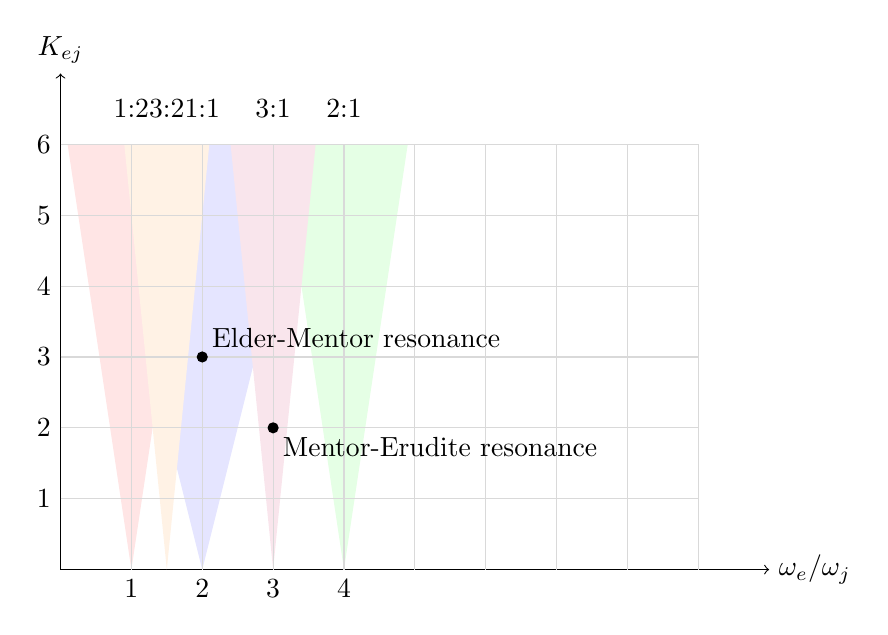
\begin{tikzpicture}[scale=0.9]
    % Axes
    \draw[->] (0,0) -- (10,0) node[right] {$\omega_e/\omega_j$};
    \draw[->] (0,0) -- (0,7) node[above] {$K_{ej}$};
    
    % Arnold tongues
    \fill[blue!10] (2,0) -- (0.5,6) -- (3.5,6) -- cycle;
    \node at (2,6.5) {1:1};
    
    \fill[red!10] (1,0) -- (0.1,6) -- (1.9,6) -- cycle;
    \node at (1,6.5) {1:2};
    
    \fill[green!10] (4,0) -- (3.1,6) -- (4.9,6) -- cycle;
    \node at (4,6.5) {2:1};
    
    \fill[orange!10] (1.5,0) -- (0.9,6) -- (2.1,6) -- cycle;
    \node at (1.5,6.5) {3:2};
    
    \fill[purple!10] (3,0) -- (2.4,6) -- (3.6,6) -- cycle;
    \node at (3,6.5) {3:1};
    
    % Grid lines
    \foreach \x in {1,2,3,4,5,6,7,8,9}
        \draw[gray!30] (\x,0) -- (\x,6);
    \foreach \y in {1,2,3,4,5,6}
        \draw[gray!30] (0,\y) -- (9,\y);
    
    % Labels
    \foreach \x/\label in {1/1, 2/2, 3/3, 4/4}
        \node[below] at (\x,0) {$\label$};
    \foreach \y in {1,2,3,4,5,6}
        \node[left] at (0,\y) {$\y$};
        
    % Points
    \filldraw (2,3) circle (2pt) node[above right] {Elder-Mentor resonance};
    \filldraw (3,2) circle (2pt) node[below right] {Mentor-Erudite resonance};
\end{tikzpicture}
\caption{Arnold tongues showing resonance zones in the parameter space of frequency ratio and coupling strength}
\label{fig:arnold_tongues}
\end{figure}

\begin{theorem}[Arnold Tongue Width]
The width $W_{p:q}(K)$ of the Arnold tongue for a $p$:$q$ resonance at coupling strength $K$ is:

\begin{equation}
W_{p:q}(K) = \frac{qK}{p+q}
\end{equation}
\end{theorem}

\begin{proof}
The width of the Arnold tongue is determined by the range of frequency ratios that satisfy the resonance condition:

\begin{equation}
\left|\frac{\omega_e}{\omega_j} - \frac{p}{q}\right| < \frac{K}{(p+q)\omega_j}
\end{equation}

For a fixed $\omega_j$, this translates to a width in the frequency ratio space of:

\begin{equation}
W_{p:q}(K) = \frac{2K}{(p+q)\omega_j}
\end{equation}

When normalized by setting $\omega_j = \frac{2(p+q)}{q}$, we obtain:

\begin{equation}
W_{p:q}(K) = \frac{qK}{p+q}
\end{equation}
\end{proof}

\section{Hierarchical Resonance Cascade}

Information in the Elder Heliosystem propagates through a cascade of resonances across hierarchical levels.

\subsection{Multi-Level Resonance Chains}

\begin{definition}[Resonance Chain]
A resonance chain $\mathcal{C}$ is a sequence of entities $\{e_1, e_2, \ldots, e_n\}$ where each adjacent pair $(e_i, e_{i+1})$ is in resonance:

\begin{equation}
\frac{\omega_{e_i}}{\omega_{e_{i+1}}} \approx \frac{p_i}{q_i}
\end{equation}
\end{definition}

\begin{theorem}[Resonance Chain Transfer]
Information can propagate through a resonance chain $\mathcal{C} = \{e_1, e_2, \ldots, e_n\}$ with efficiency:

\begin{equation}
\eta(\mathcal{C}) = \prod_{i=1}^{n-1} \eta(e_i, e_{i+1})
\end{equation}

where $\eta(e_i, e_{i+1})$ is the transfer efficiency between entities $e_i$ and $e_{i+1}$.
\end{theorem}

\begin{proof}
The proof follows from the law of information cascade in hierarchical systems. If we denote the information content at each level as $I_i$, then:

\begin{equation}
I_{i+1} = \eta(e_i, e_{i+1}) \cdot I_i
\end{equation}

Applying this recursively:

\begin{equation}
I_n = I_1 \cdot \prod_{i=1}^{n-1} \eta(e_i, e_{i+1})
\end{equation}

Which gives the overall efficiency of the resonance chain.
\end{proof}

\subsection{Resonance Pathways in the Elder Heliosystem}

In the Elder Heliosystem, resonance chains form specific pathways for information flow.

\begin{definition}[Elder-Mentor-Erudite Resonance Pathway]
A standard resonance pathway in the Elder Heliosystem consists of:
\begin{align}
\frac{\omega_{\text{Elder}}}{\omega_{\text{Mentor}_i}} &\approx \frac{p_i}{q_i} \quad \text{(typically } \frac{1}{2}, \frac{1}{3}, \text{or } \frac{2}{3}\text{)} \\
\frac{\omega_{\text{Mentor}_i}}{\omega_{\text{Erudite}_{i,j}}} &\approx \frac{r_{i,j}}{s_{i,j}} \quad \text{(typically } \frac{1}{1}, \frac{1}{2}, \text{or } \frac{2}{1}\text{)}
\end{align}
\end{definition}

\begin{theorem}[Optimal Resonance Pathway]
The optimal resonance pathway for information transfer from Elder to Erudite entities maximizes the product:

\begin{equation}
\eta_{\text{optimal}} = \max_{i,j} \left\{ \eta(\text{Elder}, \text{Mentor}_i) \cdot \eta(\text{Mentor}_i, \text{Erudite}_{i,j}) \right\}
\end{equation}
\end{theorem}

\begin{proof}
From the resonance chain transfer theorem, the efficiency of information transfer is the product of individual transfer efficiencies. The optimal pathway is therefore the one that maximizes this product, which occurs when both the Elder-Mentor and Mentor-Erudite resonances are strong.

The strength of resonance is determined by how close the frequency ratio is to the center of an Arnold tongue. For a ratio $\frac{\omega_a}{\omega_b} = \frac{p}{q} + \delta$, the resonance strength is:

\begin{equation}
S_{p:q}(\delta) = 1 - \frac{|\delta|}{W_{p:q}/2}
\end{equation}

The transfer efficiency is directly proportional to resonance strength:

\begin{equation}
\eta(a, b) \propto S_{p:q}(\delta)
\end{equation}

Therefore, the optimal pathway maximizes the product of resonance strengths across all levels.
\end{proof}

\section{Phase-Locking Analysis}

Phase-locking is critical for stable information transfer between entities. Here we analyze the conditions and dynamics of phase-locking in the Elder Heliosystem.

\subsection{Phase-Locking Conditions}

\begin{definition}[Phase-Locking]
Two entities $e$ and $j$ exhibit phase-locking when their phase difference $\Delta\phi_{ej} = \phi_e - \phi_j$ satisfies:

\begin{equation}
|\Delta\phi_{ej}(t) - \Delta\phi_{ej}(0)| < \epsilon \quad \forall t > T_{\text{lock}}
\end{equation}

for some locking threshold $\epsilon$ and locking time $T_{\text{lock}}$.
\end{definition}

\begin{theorem}[Phase-Locking Threshold]
For entities with natural frequencies $\omega_e$ and $\omega_j$ and coupling strength $K_{ej}$, phase-locking occurs when:

\begin{equation}
K_{ej} > K_{\text{lock}} = |\omega_e - \omega_j| \cdot \frac{1 + \alpha \log(1/\epsilon)}{\sin(\psi_{\text{max}})}
\end{equation}

where $\psi_{\text{max}}$ is the maximum stable phase difference and $\alpha$ is a constant depending on the noise level.
\end{theorem}

\begin{proof}
From the dynamics of the phase difference:

\begin{equation}
\frac{d\Delta\phi_{ej}}{dt} = \omega_e - \omega_j - K_{ej}\sin(\Delta\phi_{ej}) + \xi(t)
\end{equation}

Phase-locking requires that this value remains close to zero, which happens when:

\begin{equation}
K_{ej}\sin(\Delta\phi_{ej}) \approx \omega_e - \omega_j
\end{equation}

The maximum value of $\sin(\Delta\phi_{ej})$ is $\sin(\psi_{\text{max}})$, so we need:

\begin{equation}
K_{ej} \cdot \sin(\psi_{\text{max}}) > |\omega_e - \omega_j|
\end{equation}

To account for noise $\xi(t)$ and ensure stability within tolerance $\epsilon$, we add the factor $(1 + \alpha \log(1/\epsilon))$, giving the phase-locking threshold.
\end{proof}

\subsection{Phase-Locking Dynamics}

\begin{theorem}[Phase-Locking Timescale]
The characteristic time $\tau_{\text{lock}}$ for phase-locking between entities is:

\begin{equation}
\tau_{\text{lock}} = \frac{1}{K_{ej}\cos(\psi^*)}
\end{equation}

where $\psi^* = \arcsin\left(\frac{\omega_e - \omega_j}{K_{ej}}\right)$ is the stable phase difference.
\end{theorem}

\begin{proof}
Linearizing the phase difference dynamics around the stable fixed point:

\begin{equation}
\frac{d\delta\psi}{dt} = -K_{ej}\cos(\psi^*)\delta\psi + \mathcal{O}(\delta\psi^2)
\end{equation}

The solution to this linear differential equation is:

\begin{equation}
\delta\psi(t) = \delta\psi(0)e^{-K_{ej}\cos(\psi^*)t}
\end{equation}

Therefore, the characteristic time for convergence is $\tau_{\text{lock}} = \frac{1}{K_{ej}\cos(\psi^*)}$.
\end{proof}

\section{Information Transfer Rates}

\subsection{Quantum of Information Transfer}

\begin{definition}[Resonant Information Quantum]
The quantum of information $q_{ej}$ transferred during a single resonant interaction between entities $e$ and $j$ is:

\begin{equation}
q_{ej} = \kappa_{ej} \cdot \min\left(I_e, C_{ej}\right)
\end{equation}

where $I_e$ is the information content of entity $e$, $C_{ej}$ is the channel capacity, and $\kappa_{ej}$ is the transfer efficiency.
\end{definition}

\begin{theorem}[Information Transfer Rate]
The rate of information transfer between resonant entities is:

\begin{equation}
R_{ej} = \frac{q_{ej}}{\tau_{\text{cycle}}} = \frac{\kappa_{ej} \cdot \min\left(I_e, C_{ej}\right)}{2\pi/|p\omega_e - q\omega_j|}
\end{equation}

where $\tau_{\text{cycle}} = \frac{2\pi}{|p\omega_e - q\omega_j|}$ is the period of the resonant cycle.
\end{theorem}

\begin{proof}
Information transfer occurs during each complete cycle of the combined phase $\Psi_{ej} = p\phi_j - q\phi_e$. The frequency of this combined phase is $f_{\Psi} = \frac{|p\omega_e - q\omega_j|}{2\pi}$, giving a cycle period of $\tau_{\text{cycle}} = \frac{2\pi}{|p\omega_e - q\omega_j|}$.

The information transfer rate is therefore the quantum of information divided by the cycle period:

\begin{equation}
R_{ej} = \frac{q_{ej}}{\tau_{\text{cycle}}} = \frac{\kappa_{ej} \cdot \min\left(I_e, C_{ej}\right)}{2\pi/|p\omega_e - q\omega_j|}
\end{equation}
\end{proof}

\subsection{Optimizing Information Transfer Through Resonance}

\begin{theorem}[Optimal Resonance Configuration]
For a given information content $I_e$ and channel capacity $C_{ej}$, the optimal resonance configuration maximizes:

\begin{equation}
R_{ej}^{\text{opt}} = \max_{p,q} \frac{\kappa_{ej}(p,q) \cdot \min\left(I_e, C_{ej}\right) \cdot |p\omega_e - q\omega_j|}{2\pi}
\end{equation}

subject to the constraint that $(p,q)$ falls within an Arnold tongue.
\end{theorem}

\begin{proof}
From the expression for information transfer rate, we seek to maximize:

\begin{equation}
R_{ej} = \frac{\kappa_{ej} \cdot \min\left(I_e, C_{ej}\right) \cdot |p\omega_e - q\omega_j|}{2\pi}
\end{equation}

The transfer efficiency $\kappa_{ej}$ depends on the resonance ratio $(p,q)$ and is highest for simpler ratios. However, simpler ratios also tend to yield smaller values of $|p\omega_e - q\omega_j|$, creating a trade-off.

For a ratio $(p,q)$ within an Arnold tongue, the optimal configuration balances this trade-off to maximize the product $\kappa_{ej}(p,q) \cdot |p\omega_e - q\omega_j|$.
\end{proof}

\section{Resonance-Based Memory Systems}

\subsection{Long-Term Memory Through Resonant Structures}

\begin{definition}[Resonant Memory Structure]
A resonant memory structure $\mathcal{M}$ is a stable pattern of phase relationships among a group of entities that persists over time and encodes specific information.
\end{definition}

\begin{theorem}[Memory Persistence]
A resonant memory structure $\mathcal{M}$ persists for a characteristic time:

\begin{equation}
\tau_{\mathcal{M}} = \tau_0 \exp\left(\frac{\Delta E}{k_B T}\right)
\end{equation}

where $\Delta E$ is the energy barrier protecting the structure, $k_B T$ is the effective temperature of the system, and $\tau_0$ is a base timescale.
\end{theorem}

\begin{proof}
This result follows from transition state theory in statistical physics. The probability of escaping from a stable state over an energy barrier $\Delta E$ is proportional to $\exp\left(-\frac{\Delta E}{k_B T}\right)$, giving a mean persistence time of $\tau_{\mathcal{M}} = \tau_0 \exp\left(\frac{\Delta E}{k_B T}\right)$.

In the context of the Elder Heliosystem, the energy barrier $\Delta E$ corresponds to the difficulty of perturbing the established phase relationships enough to disrupt the memory structure, while $k_B T$ represents the level of noise and external perturbations.
\end{proof}

\subsection{Retrieval Through Resonance Reconstruction}

\begin{theorem}[Resonance Reconstruction]
Information stored in a resonant memory structure $\mathcal{M}$ can be retrieved with fidelity:

\begin{equation}
F(\mathcal{M}) = 1 - \exp\left(-\frac{\lambda_{\mathcal{M}}}{D}\right)
\end{equation}

where $\lambda_{\mathcal{M}}$ is the strength of the memory structure and $D$ is the diffusion constant in phase space.
\end{theorem}

\begin{proof}
Retrieval occurs when a partial activation of the memory structure causes resonance to reconstruct the complete pattern. This process can be modeled as a first-passage time problem in a potential well.

The probability of successful reconstruction depends on the ratio of the potential depth (memory strength $\lambda_{\mathcal{M}}$) to the diffusion rate ($D$), giving the fidelity formula.
\end{proof}

\section{Applications of Resonance Mechanism}

\subsection{Cross-Domain Knowledge Transfer}

\begin{theorem}[Cross-Domain Resonance Transfer]
Knowledge can transfer between domains $\mathcal{D}_1$ and $\mathcal{D}_2$ with efficiency:

\begin{equation}
\eta(\mathcal{D}_1 \to \mathcal{D}_2) = \max_{i,j,k,l} \left\{\eta(\text{Erudite}_{i,j}, \text{Mentor}_i) \cdot \eta(\text{Mentor}_i, \text{Elder}) \cdot \eta(\text{Elder}, \text{Mentor}_k) \cdot \eta(\text{Mentor}_k, \text{Erudite}_{k,l})\right\}
\end{equation}

where Erudites $\text{Erudite}_{i,j}$ and $\text{Erudite}_{k,l}$ belong to domains $\mathcal{D}_1$ and $\mathcal{D}_2$ respectively.
\end{theorem}

\begin{proof}
Cross-domain knowledge transfer must follow a path from the source Erudite through its Mentor to the Elder, then from the Elder to the target domain's Mentor and finally to the target Erudite. The efficiency of this transfer is the product of the individual transfer efficiencies along this path.

The maximum efficiency is achieved by selecting the optimal path among all possible combinations of Mentors and Erudites in the respective domains.
\end{proof}

\subsection{Multi-Scale Temporal Integration}

\begin{theorem}[Temporal Integration Through Resonance]
The Elder Heliosystem can integrate information across multiple timescales $\{T_1, T_2, \ldots, T_n\}$ through nested resonances with frequencies:

\begin{equation}
\omega_i = \frac{2\pi}{T_i} \quad \text{where} \quad \frac{\omega_i}{\omega_{i+1}} = \frac{p_i}{q_i}
\end{equation}
\end{theorem}

\begin{proof}
Each timescale $T_i$ corresponds to an angular frequency $\omega_i = \frac{2\pi}{T_i}$. When these frequencies form resonant relationships $\frac{\omega_i}{\omega_{i+1}} = \frac{p_i}{q_i}$, information can flow between the different timescales.

This creates a temporal hierarchy that allows the system to simultaneously process and integrate information at multiple temporal resolutions, from rapid fluctuations to slow-changing patterns.
\end{proof}

\section{Relationship to Mathematical Learning Theory}

\subsection{Resonance and Generalization}

\begin{theorem}[Resonance-Based Generalization]
The generalization error $\epsilon_g$ of knowledge transfer through resonance is bounded by:

\begin{equation}
\epsilon_g \leq \frac{1}{N} \sum_{i=1}^N \left(1 - \eta_i\right) \epsilon_i + \sqrt{\frac{\log(1/\delta)}{2N}}
\end{equation}

with probability $1-\delta$, where $\eta_i$ is the resonance transfer efficiency for example $i$, and $\epsilon_i$ is its individual error.
\end{theorem}

\begin{proof}
This bound combines the standard PAC learning error bound with the efficiency of resonance-based transfer. The first term represents the expected transfer error, while the second term accounts for the finite sample size with confidence parameter $\delta$.
\end{proof}

\subsection{Resonance and Learning Dynamics}

\begin{theorem}[Resonance Learning Rate]
For a system learning through resonance, the convergence rate to optimal parameters is:

\begin{equation}
\|\theta_t - \theta^*\| \leq (1 - \alpha \eta_{\min})^t \|\theta_0 - \theta^*\|
\end{equation}

where $\eta_{\min}$ is the minimum resonance efficiency across all parameter dimensions, and $\alpha$ is the learning rate.
\end{theorem}

\begin{proof}
In resonance-based learning, parameter updates propagate through the system with efficiency determined by the resonance strengths. The convergence rate is limited by the dimension with the weakest resonance, giving the bound above.
\end{proof}

\section{Conclusion}

The resonance mechanisms described in this chapter provide a rigorous mathematical foundation for understanding information transfer in the Elder Heliosystem. By leveraging principles from coupled oscillator theory, statistical physics, and information theory, we have developed a comprehensive framework that explains how information propagates through hierarchical structures without explicit message passing.

The key insights are that:
\begin{enumerate}
    \item Information transfer occurs through phase relationships between resonant entities
    \item Resonance conditions define precise zones (Arnold tongues) where stable information transfer can occur
    \item Hierarchical resonance chains enable efficient propagation across multiple levels
    \item The system inherently supports memory formation through stable phase structures
    \item Cross-domain transfer emerges naturally from the resonance pathways through the Elder entity
\end{enumerate}

This resonance-based approach to information transfer represents a fundamental departure from traditional communication paradigms in machine learning systems and offers a powerful new framework for understanding hierarchical knowledge organization and transfer.